\let\negmedspace\undefined
\let\negthickspace\undefined
\documentclass[journal,12pt,onecolumn]{IEEEtran}
\usepackage{cite}
\usepackage{amsmath,amssymb,amsfonts,amsthm}
\usepackage{algorithmic}
\usepackage{amsmath}
\usepackage{graphicx}
\graphicspath{{./figs/}}
\usepackage{textcomp}
\usepackage{framed} 

\usepackage[utf8]{inputenc}
\usepackage{xcolor}
\usepackage{txfonts}
\usepackage{romannum}
\usepackage{listings}
\usepackage{enumitem}
\usepackage{mathtools}
\usepackage{gensymb}
\usepackage{comment}
\usepackage{caption}
\usepackage[breaklinks=true]{hyperref}
\usepackage{tkz-euclide} 
\usepackage{listings}
\usepackage{gvv}                                        
\usepackage{color}        
\usepackage[utf8]{inputenc}                                     
\usepackage{array}                                            
\usepackage{longtable}         
\usepackage{multicol}                              
\usepackage{calc}                                             
\usepackage{multirow}
\usepackage{multicol}
\usepackage{hhline}                                           
\usepackage{ifthen}                                           
\usepackage{lscape}
\usepackage{tabularx}
\usepackage{array}
\usepackage{float}
\newtheorem{theorem}{Theorem}[section]
\newtheorem{problem}{Problem}
\newtheorem{proposition}{Proposition}[section]
\newtheorem{lemma}{Lemma}[section]
\newtheorem{corollary}[theorem]{Corollary}
\newtheorem{example}{Example}[section]
\newtheorem{definition}[problem]{Definition}
\newcommand{\BEQA}{\begin{eqnarray}}
	\newcommand{\EEQA}{\end{eqnarray}}

\theoremstyle{remark}
\begin{document}
		\title{GATE CS 2016 SET-1}
	\author{EE25BTECH11052 - Shriyansh Chawda}
	\maketitle
	\fbox{{\large Q.1 - Q.5 Carry ONE mark each}}\\
	\begin{enumerate}
		
		\item Out of the following four sentences, select the most suitable sentence with respect to grammar and usage.
		
		\hfill{\brak{\text{GATE CS 2016}}}
		\begin{enumerate}
			\begin{multicols}{2}
				\item I will not leave the place until the minister does not meet me.
				\item I will not leave the place until the minister doesn't meet me.
				\item I will not leave the place until the minister meet me.
				\item I will not leave the place until the minister meets me.
			\end{multicols}
		\end{enumerate}
		
		\item A rewording of something written or spoken is a \underline{\hspace{2cm}}.
		
		\hfill{\brak{\text{GATE CS 2016}}}
		\begin{enumerate}
			\begin{multicols}{4}
				\item paraphrase
				\item paradox
				\item paradigm
				\item paraffin
			\end{multicols}
		\end{enumerate}
		
		\item Archimedes said, "Give me a lever long enough and a fulcrum on which to place it, and I will move the world."
		The sentence above is an example of a \underline{\hspace{2cm}} statement.
		
		\hfill{\brak{\text{GATE CS 2016}}}
		\begin{enumerate}
			\begin{multicols}{4}
				\item figurative
				\item collateral
				\item literal
				\item figurine
			\end{multicols}
		\end{enumerate}
		
		\item If 'relftaga' means carefree, 'otaga' means careful and 'fertaga' means careless, which of the following could mean 'aftercare'?
		
		\hfill{\brak{\text{GATE CS 2016}}}
		\begin{enumerate}
			\begin{multicols}{4}
				\item zentaga
				\item tagafer
				\item tagazen
				\item relffer
			\end{multicols}
		\end{enumerate}
		
		\item A cube is built using $64$ cubic blocks of side one unit. After it is built, one cubic block is removed from every corner of the cube. The resulting surface area of the body $\brak{\text{in square units}}$ after the removal is \underline{\hspace{2cm}}.
		
		\hfill{\brak{\text{GATE CS 2016}}}
		\begin{enumerate}
			\begin{multicols}{4}
				\item $56$
				\item $64$
				\item $72$
				\item $96$
			\end{multicols}
		\end{enumerate}
		
		\item A shaving set company sells $4$ different types of razors, Elegance, Smooth, Soft and Executive. Elegance sells at Rs. $48$, Smooth at Rs. $63$, Soft at Rs. $78$ and Executive at Rs. $173$ per piece. The table below shows the numbers of each razor sold in each quarter of a year.
		
		\begin{table}[h]
			\centering
			\begin{tabular}{|l|c|c|c|c|}
				\hline
				Quarter \textbackslash Product & Elegance & Smooth & Soft & Executive \\
				\hline
				Q1 & 27300 & 20009 & 17602 & 9999 \\
								\hline
				Q2 & 25222 & 19392 & 18445 & 8942 \\
								\hline
				Q3 & 28976 & 22429 & 19544 & 10234 \\
								\hline
				Q4 & 21012 & 18229 & 16595 & 10109 \\
				
				\hline
			\end{tabular}
			\caption*{}
			\label{tab:razorsales}
		\end{table}
		
		Which product contributes the greatest fraction to the revenue of the company in that year?
		
		\hfill{\brak{\text{GATE CS 2016}}}
		\begin{enumerate}
			\begin{multicols}{4}
				\item Elegance
				\item Executive
				\item Smooth
				\item Soft
			\end{multicols}
		\end{enumerate}
		
		\item Indian currency notes show the denomination indicated in at least seventeen languages. If this is not an indication of the nation's diversity, nothing else is.
		Which of the following can be logically inferred from the above sentences?
		
		\hfill{\brak{\text{GATE CS 2016}}}
		\begin{enumerate}
			\item India is a country of exactly seventeen languages.
			\item Linguistic pluralism is the only indicator of a nation's diversity.
			\item Indian currency notes have sufficient space for all the Indian languages.
			\item Linguistic pluralism is strong evidence of India's diversity.
		\end{enumerate}
		
		\item Consider the following statements relating to the level of poker play of four players P, Q, R and S.
		\begin{enumerate}
			\item \textbf{P} always beats \textbf{Q}
			\item \textbf{R} always beats \textbf{S}
			\item \textbf{S} loses to P only sometimes
			\item \textbf{R} always loses to \textbf{Q}
		\end{enumerate}
		Which of the following can be logically inferred from the above statements?
		\begin{enumerate}
			\item \textbf{P} is likely to beat all the three other players
			\item \textbf{S} is the absolute worst player in the set
		\end{enumerate}
		
		\hfill{\brak{\text{GATE CS 2016}}}
		\begin{enumerate}
			\begin{multicols}{4}
				\item $\brak{\text{i}}$ only
				\item $\brak{\text{ii}}$ only
				\item $\brak{\text{i}}$ and $\brak{\text{ii}}$
				\item neither $\brak{\text{i}}$ nor $\brak{\text{ii}}$
			\end{multicols}
		\end{enumerate}
		
		\item If $f\brak{x} = 2x^7 + 3x - 5$, which of the following is a factor of $f\brak{x}$?
		
		\hfill{\brak{\text{GATE CS 2016}}}
		\begin{enumerate}
			\begin{multicols}{4}
				\item $\brak{x^3 + 8}$
				\item $\brak{x - 1}$
				\item $\brak{2x - 5}$
				\item $\brak{x + 1}$
			\end{multicols}
		\end{enumerate}
		
		\item In a process, the number of cycles to failure decreases exponentially with an increase in load. At a load of $80$ units, it takes $100$ cycles for failure. When the load is halved, it takes $10000$ cycles for failure. The load for which the failure will happen in $5000$ cycles is \underline{\hspace{2cm}}.
		
		\hfill{\brak{\text{GATE CS 2016}}}
		\begin{enumerate}
			\begin{multicols}{4}
				\item $40.00$
				\item $46.02$
				\item $60.01$
				\item $92.02$
			\end{multicols}
		\end{enumerate}
	\end{enumerate}
	\newpage
		\fbox{{\large Q. 1 - Q. 25 carry one mark each}}\\
	\begin{enumerate}


		
		\item Let $p$, $q$, $r$, $s$ represent the following propositions.
		\begin{align*}
			p\colon & \quad x \in \{8, 9, 10, 11, 12\} \\
			q\colon & \quad x \text{ is a composite number} \\
			r\colon & \quad x \text{ is a perfect square} \\
			s\colon & \quad x \text{ is a prime number}
		\end{align*}
		The integer $x \geq 2$ which satisfies $\neg\brak{\brak{p \Rightarrow q} \land \brak{\neg r \lor \neg s}}$ is \underline{\hspace{2cm}}.
		
		\hfill{\brak{\text{GATE CS 2016}}}
		
		\item Let $a_n$ be the number of $n$-bit strings that do NOT contain two consecutive $1$s. Which one of the following is the recurrence relation for $a_n$?
		
		\hfill{\brak{\text{GATE CS 2016}}}
		\begin{enumerate}
			\begin{multicols}{2}
				\item $a_n = a_{n-1} + 2a_{n-2}$
				\item $a_n = a_{n-1} + a_{n-2}$
				\item $a_n = 2a_{n-1} + a_{n-2}$
				\item $a_n = 2a_{n-1} + 2a_{n-2}$
			\end{multicols}
		\end{enumerate}
		
		\item $\lim_{x \to 4} \frac{\sin\brak{x - 4}}{x - 4} = $ \underline{\hspace{2cm}}.
		
		\hfill{\brak{\text{GATE CS 2016}}}
		
		\item A probability density function on the interval $[a, 1]$ is given by $1/x^2$ and outside this interval the value of the function is zero. The value of $a$ is \underline{\hspace{2cm}}.
		
		\hfill{\brak{\text{GATE CS 2016}}}
		
		\item Two eigenvalues of a $3 \times 3$ real matrix $P$ are $\brak{2 + \sqrt{-1}}$ and $3$. The determinant of $P$ is \underline{\hspace{2cm}}.
		
		\hfill{\brak{\text{GATE CS 2016}}}
		
		\item Consider the Boolean operator $\#$ with the following properties:
		$x \# 0 = x$, $x \# 1 = \bar{x}$, $x \# x = 0$ and $x \# \bar{x} = 1$. Then $x \# y$ is equivalent to
		
		\hfill{\brak{\text{GATE CS 2016}}}
		\begin{enumerate}
			\begin{multicols}{4}
				\item $x\bar{y} + \bar{x}y$
				\item $x\bar{y} + \bar{x}\bar{y}$
				\item $\bar{x}y + xy$
				\item $xy + \bar{x}\bar{y}$
			\end{multicols}
		\end{enumerate}
		
		\item The $16$-bit $2$'s complement representation of an integer is $1111$ $1111$ $1111$ $0101$; its decimal representation is \underline{\hspace{2cm}}.
		
		\hfill{\brak{\text{GATE CS 2016}}}
		
		\item We want to design a synchronous counter that counts the sequence $0$-$1$-$0$-$2$-$0$-$3$ and then repeats. The minimum number of J-K flip-flops required to implement this counter is \underline{\hspace{2cm}}.
		
		\hfill{\brak{\text{GATE CS 2016}}}
		
		\item A processor can support a maximum memory of $4$ GB, where the memory is word-addressable $\brak{\text{a word consists of two bytes}}$. The size of the address bus of the processor is at least \underline{\hspace{2cm}} bits.
		
		\hfill{\brak{\text{GATE CS 2016}}}
		
		\item A queue is implemented using an array such that ENQUEUE and DEQUEUE operations are performed efficiently. Which one of the following statements is CORRECT $\brak{n \text{ refers to the number of items in the queue}}$?
		
		\hfill{\brak{\text{GATE CS 2016}}}
		\begin{enumerate}
			\item Both operations can be performed in $O\brak{1}$ time
			\item At most one operation can be performed in $O\brak{1}$ time but the worst case time for the other operation will be $\Omega\brak{n}$
			\item The worst case time complexity for both operations will be $\Omega\brak{n}$
			\item Worst case time complexity for both operations will be $\Omega\brak{\log n}$
		\end{enumerate}
		
		\item Consider the following directed graph:
		
	\begin{figure}[H]
		\centering
		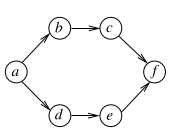
\includegraphics[width=0.3\linewidth]{screenshot001}
		\caption{}
		\label{fig:screenshot001}
	\end{figure}
	
		
		The number of different topological orderings of the vertices of the graph is \underline{\hspace{2cm}}.
		
		\hfill{\brak{\text{GATE CS 2016}}}
		
		\item Consider the following C program.
		\begin{verbatim}
			void f(int, short);
			void main()
			{
				int i = 100;
				short s = 12;
				short *p = &s;
				__________ ; // call to f()
			}
		\end{verbatim}
		Which one of the following expressions, when placed in the blank above, will NOT result in a type checking error?
		
		\hfill{\brak{\text{GATE CS 2016}}}
		\begin{enumerate}
			\begin{multicols}{4}
				\item f$\brak{\text{s,*s}}$
				\item i = f$\brak{\text{i,s}}$
				\item f$\brak{\text{i,*s}}$
				\item f$\brak{\text{i,*p}}$
			\end{multicols}
		\end{enumerate}
		
		\item The worst case running times of Insertion sort, Merge sort and Quick sort, respectively, are:
		
		\hfill{\brak{\text{GATE CS 2016}}}
		\begin{enumerate}
				\begin{multicols}{2}
			\item $\Theta\brak{n \log n}$, $\Theta\brak{n \log n}$, and $\Theta\brak{n^2}$
			\item $\Theta\brak{n^2}$, $\Theta\brak{n^2}$, and $\Theta\brak{n \log n}$
			\item $\Theta\brak{n^2}$, $\Theta\brak{n \log n}$, and $\Theta\brak{n \log n}$
			\item $\Theta\brak{n^2}$, $\Theta\brak{n \log n}$, and $\Theta\brak{n^2}$						\end{multicols}
		\end{enumerate}
		
		\item Let $G$ be a weighted connected undirected graph with distinct positive edge weights. If every edge weight is increased by the same value, then which of the following statements is/are TRUE?
		\begin{align*}
			P\colon & \text{ Minimum spanning tree of } G \text{ does not change} \\
			Q\colon & \text{ Shortest path between any pair of vertices does not change}
		\end{align*}
		
		\hfill{\brak{\text{GATE CS 2016}}}
		\begin{enumerate}
			\begin{multicols}{4}
				\item P only
				\item Q only
				\item Neither P nor Q
				\item Both P and Q
			\end{multicols}
		\end{enumerate}
		
		\item Consider the following C program.
		\begin{verbatim}
			#include<stdio.h>
			void mystery(int *ptra, int *ptrb) {
				int *temp;
				temp = ptrb;
				ptrb = ptra;
				ptra = temp;
			}
			int main() {
				int a=2016, b=0, c=4, d=42;
				mystery(&a, &b);
				if (a < c)
				mystery(&c, &a);
				mystery(&a, &d);
				printf("%d\n", a);
			}
		\end{verbatim}
		The output of the program is \underline{\hspace{2cm}}.
		
		\hfill{\brak{\text{GATE CS 2016}}}
		
		\item Which of the following languages is generated by the given grammar?
		\begin{align*}
			S \rightarrow aS \mid bS \mid \varepsilon
		\end{align*}
		
		\hfill{\brak{\text{GATE CS 2016}}}
		\begin{enumerate}
		

			\item $\{a^n b^m \mid n, m \geq 0\}$
			\item $\{w \in \{a, b\}^* \mid w \text{ has equal number of a's and b's}\}$ 
			\item $\{a^n \mid n \geq 0\} \cup \{b^n \mid n \geq 0\} \cup \{a^n b^n \mid n \geq 0\}$
			\item $\{a, b\}^*$

		\end{enumerate}
		
		\item Which of the following decision problems are undecidable?
		\begin{enumerate}
			\item Given NFAs $N_1$ and $N_2$, is $L\brak{N_1} \cap L\brak{N_2} = \Phi$?
			\item Given a CFG $G = \brak{N, \Sigma, P, S}$ and a string $x \in \Sigma^*$, does $x \in L\brak{G}$?
			\item Given CFGs $G_1$ and $G_2$, is $L\brak{G_1} = L\brak{G_2}$?
			\item Given a TM $M$, is $L\brak{M} = \Phi$?
		\end{enumerate}
		
		\hfill{\brak{\text{GATE CS 2016}}}
		\begin{enumerate}
			\begin{multicols}{4}
				\item I and IV only
				\item II and III only
				\item III and IV only
				\item II and IV only
			\end{multicols}
		\end{enumerate}
		
		\item Which one of the following regular expressions represents the language: the set of all binary strings having two consecutive $0$s and two consecutive $1$s?
		
		\hfill{\brak{\text{GATE CS 2016}}}
		\begin{enumerate}
			\item $\brak{0 + 1}^* 0011 \brak{0 + 1}^* + \brak{0 + 1}^* 1100 \brak{0 + 1}^*$
			\item $\brak{0 + 1}^* \brak{00\brak{0 + 1}^* 11 + 11\brak{0 + 1}^* 00} \brak{0 + 1}^*$
			\item $\brak{0 + 1}^* 00 \brak{0 + 1}^* + \brak{0 + 1}^* 11 \brak{0 + 1}^*$
			\item $00\brak{0 + 1}^* 11 + 11\brak{0 + 1}^* 00$
		\end{enumerate}
		
		\item Consider the following code segment.
		\begin{verbatim}
			x = u - t;
			y = x * v;
			x = y + w;
			y = t - z;
			y = x * y;
		\end{verbatim}
		The minimum number of total variables required to convert the above code segment to static single assignment form is \underline{\hspace{2cm}}.
		
		\hfill{\brak{\text{GATE CS 2016}}}
		
		\item Consider an arbitrary set of CPU-bound processes with unequal CPU burst lengths submitted at the same time to a computer system. Which one of the following process scheduling algorithms would minimize the average waiting time in the ready queue?
		
		\hfill{\brak{\text{GATE CS 2016}}}
		\begin{enumerate}
			\item Shortest remaining time first
			\item Round-robin with time quantum less than the shortest CPU burst
			\item Uniform random
			\item Highest priority first with priority proportional to CPU burst length
		\end{enumerate}
		
		\item Which of the following is NOT a superkey in a relational schema with attributes $V, W, X, Y, Z$ and primary key $VY$?
		
		\hfill{\brak{\text{GATE CS 2016}}}
		\begin{enumerate}
			\begin{multicols}{4}
				\item $VXYZ$
				\item $VWXZ$
				\item $VWXY$
				\item $VWXYZ$
			\end{multicols}
		\end{enumerate}
		
		\item Which one of the following is NOT a part of the ACID properties of database transactions?
		
		\hfill{\brak{\text{GATE CS 2016}}}
		\begin{enumerate}
			\begin{multicols}{4}
				\item Atomicity
				\item Consistency
				\item Isolation
				\item Deadlock-freedom
			\end{multicols}
		\end{enumerate}
		
		\item A database of research articles in a journal uses the following schema.
		$\brak{\text{VOLUME, NUMBER, STARTPAGE, ENDPAGE, TITLE, YEAR, PRICE}}$
		The primary key is $\brak{\text{VOLUME, NUMBER, STARTPAGE, ENDPAGE}}$ and the following functional dependencies exist in the schema.
		\begin{align*}
			\brak{\text{VOLUME, NUMBER, STARTPAGE, ENDPAGE}} &\rightarrow \text{TITLE} \\
			\brak{\text{VOLUME, NUMBER}} &\rightarrow \text{YEAR} \\
			\brak{\text{VOLUME, NUMBER, STARTPAGE, ENDPAGE}} &\rightarrow \text{PRICE}
		\end{align*}
		The database is redesigned to use the following schemas.
		\begin{align*}
			&\brak{\text{VOLUME, NUMBER, STARTPAGE, ENDPAGE, TITLE, PRICE}} \\
			&\brak{\text{VOLUME, NUMBER, YEAR}}
		\end{align*}
		Which is the weakest normal form that the new database satisfies, but the old one does not?
		
		\hfill{\brak{\text{GATE CS 2016}}}
		\begin{enumerate}
			\begin{multicols}{4}
				\item 1NF
				\item 2NF
				\item 3NF
				\item BCNF
			\end{multicols}
		\end{enumerate}
		
		\item Which one of the following protocols is NOT used to resolve one form of address to another one?
		
		\hfill{\brak{\text{GATE CS 2016}}}
		\begin{enumerate}
			\begin{multicols}{4}
				\item DNS
				\item ARP
				\item DHCP
				\item RARP
			\end{multicols}
		\end{enumerate}
		
		\item Which of the following is/are example$\brak{\text{s}}$ of stateful application layer protocols?
		\begin{enumerate}
			\begin{multicols}{4}


			\item HTTP
			\item FTP
			\item TCP
			\item POP3			\end{multicols}
		\end{enumerate}
		
		\hfill{\brak{\text{GATE CS 2016}}}
		\begin{enumerate}
			\begin{multicols}{4}
				\item $\brak{\text{i}}$ and $\brak{\text{ii}}$ only
				\item $\brak{\text{ii}}$ and $\brak{\text{iii}}$ only
				\item $\brak{\text{ii}}$ and $\brak{\text{iv}}$ only
				\item $\brak{\text{iv}}$ only
			\end{multicols}
		\end{enumerate}
		
		\item The coefficient of $x^{12}$ in $\brak{x^3 + x^4 + x^5 + x^6 + \cdots}^3$ is \underline{\hspace{2cm}}.
		
		\hfill{\brak{\text{GATE CS 2016}}}
		
		\item Consider the recurrence relation $a_1 = 8$, $a_n = 6n^2 + 2n + a_{n-1}$. Let $a_{99} = K \times 10^4$. The value of $K$ is \underline{\hspace{2cm}}.
		
		\hfill{\brak{\text{GATE CS 2016}}}
		
		\item A function $f\colon \mathbb{N}^+ \rightarrow \mathbb{N}^+$, defined on the set of positive integers $\mathbb{N}^+$, satisfies the following properties:
		\begin{align*}
			f\brak{n} &= f\brak{n/2} \text{ if } n \text{ is even} \\
			f\brak{n} &= f\brak{n + 5} \text{ if } n \text{ is odd}
		\end{align*}
		Let $R = \{i \mid \exists j\colon f\brak{j} = i\}$ be the set of distinct values that $f$ takes. The maximum possible size of $R$ is \underline{\hspace{2cm}}.
		
		\hfill{\brak{\text{GATE CS 2016}}}
		
		\item Consider the following experiment.
		\begin{enumerate}
			\item[Step 1.] Flip a fair coin twice.
			\item[Step 2.] If the outcomes are $\brak{\text{TAILS, HEADS}}$ then output $Y$ and stop.
			\item[Step 3.] If the outcomes are either $\brak{\text{HEADS, HEADS}}$ or $\brak{\text{HEADS, TAILS}}$, then output $N$ and stop.
			\item[Step 4.] If the outcomes are $\brak{\text{TAILS, TAILS}}$, then go to Step 1.
		\end{enumerate}
		The probability that the output of the experiment is $Y$ is $\brak{\text{up to two decimal places}}$ \underline{\hspace{2cm}}.
		
		\hfill{\brak{\text{GATE CS 2016}}}
		
		\item Consider the two cascaded $2$-to-$1$ multiplexers as shown in the figure.
		
	\begin{figure}[H]
		\centering
		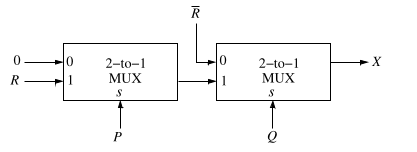
\includegraphics[width=0.5\linewidth]{figs/screenshot002}
		\caption{}
		\label{fig:screenshot002}
	\end{figure}
	
		
		The minimal sum of products form of the output $X$ is
		
		\hfill{\brak{\text{GATE CS 2016}}}
		\begin{enumerate}
			\begin{multicols}{4}
				\item $\bar{P}\bar{Q} + PQR$
				\item $\bar{P}Q + QR$
				\item $PQ + \bar{P}\bar{Q}R$
				\item $\bar{Q}\bar{R} + PQR$
			\end{multicols}
		\end{enumerate}
		
		\item The size of the data count register of a DMA controller is $16$ bits. The processor needs to transfer a file of $29,154$ kilobytes from disk to main memory. The memory is byte addressable. The minimum number of times the DMA controller needs to get the control of the system bus from the processor to transfer the file from the disk to main memory is \underline{\hspace{2cm}}.
		
		\hfill{\brak{\text{GATE CS 2016}}}
		
		\item The stage delays in a $4$-stage pipeline are $800$, $500$, $400$ and $300$ picoseconds. The first stage $\brak{\text{with delay } 800 \text{ picoseconds}}$ is replaced with a functionally equivalent design involving two stages with respective delays $600$ and $350$ picoseconds. The throughput increase of the pipeline is \underline{\hspace{2cm}} percent.
		
		\hfill{\brak{\text{GATE CS 2016}}}
		
		\item Consider a carry lookahead adder for adding two $n$-bit integers, built using gates of fan-in at most two. The time to perform addition using this adder is
		
		\hfill{\brak{\text{GATE CS 2016}}}
		\begin{enumerate}
			\begin{multicols}{4}
				\item $\Theta\brak{1}$
				\item $\Theta\brak{\log\brak{n}}$
				\item $\Theta\brak{\sqrt{n}}$
				\item $\Theta\brak{n}$
			\end{multicols}
		\end{enumerate}
		
		\item The following function computes the maximum value contained in an integer array p[] of size $n$ $\brak{n \geq 1}$.
		\begin{verbatim}
			int max(int *p, int n) {
				int a=0, b=n-1;
				while (__________) {
					if (p[a] <= p[b]) { a = a+1; }
					else { b = b-1; }
				}
				return p[a];
			}
		\end{verbatim}
		The missing loop condition is
		
		\hfill{\brak{\text{GATE CS 2016}}}
		\begin{enumerate}
			\begin{multicols}{4}
				\item a != n
				\item b != 0
				\item b $>$ $\brak{\text{a + 1}}$
				\item b != a
			\end{multicols}
		\end{enumerate}
		
		\item What will be the output of the following C program?
		\begin{verbatim}
			void count(int n){
				static int d=1;
				printf("%d ", n);
				printf("%d ", d);
				d++;
				if(n>1) count(n-1);
				printf("%d ", d);
			}
			void main(){
				count(3);
			}
		\end{verbatim}
		
		\hfill{\brak{\text{GATE CS 2016}}}
		\begin{enumerate}
			\begin{multicols}{2}
			

			\item 3 1 2 2 1 3 4 4 4
			\item 3 1 2 1 1 1 2 2 2
			\item 3 1 2 2 1 3 4
			\item 3 1 2 1 1 1 2
						\end{multicols}
		\end{enumerate}
		
		\item What will be the output of the following pseudo-code when parameters are passed by reference and dynamic scoping is assumed?
		\begin{verbatim}
			a=3;
			void n(x) {x = x * a; print(x);}
			void m(y) {a = 1; a = y - a; n(a); print(a);}
			void main() {m(a);}
		\end{verbatim}
		
		\hfill{\brak{\text{GATE CS 2016}}}
		\begin{enumerate}
			\begin{multicols}{4}
				\item 6, 2
				\item 6, 6
				\item 4, 2
				\item 4, 4
			\end{multicols}
		\end{enumerate}
		
		\item An operator delete$\brak{i}$ for a binary heap data structure is to be designed to delete the item in the $i$-th node. Assume that the heap is implemented in an array and $i$ refers to the $i$-th index of the array. If the heap tree has depth $d$ $\brak{\text{number of edges on the path from the root to the farthest leaf}}$, then what is the time complexity to re-fix the heap efficiently after the removal of the element?
		
		\hfill{\brak{\text{GATE CS 2016}}}
		\begin{enumerate}
			\begin{multicols}{2}

			\item $O\brak{1}$
			\item $O\brak{d}$ but not $O\brak{1}$
			\item $O\brak{2^d}$ but not $O\brak{d}$
			\item $O\brak{d \cdot 2^d}$ but not $O\brak{2^d}$
					\end{multicols}
				\end{enumerate}
		
		\item Consider the weighted undirected graph with $4$ vertices, where the weight of edge $\{i, j\}$ is given by the entry $W_{ij}$ in the matrix $W$.
		\[
		W = \myvec{
			0 & 2 & 8 & 5 \\
			2 & 0 & 5 & 8 \\
			8 & 5 & 0 & x \\
			5 & 8 & x & 0
		}
		\]
		The largest possible integer value of $x$, for which at least one shortest path between some pair of vertices will contain the edge with weight $x$ is \underline{\hspace{2cm}}.
		
		\hfill{\brak{\text{GATE CS 2016}}}
		
		\item Let $G$ be a complete undirected graph on $4$ vertices, having $6$ edges with weights being $1$, $2$, $3$, $4$, $5$, and $6$. The maximum possible weight that a minimum weight spanning tree of $G$ can have is \underline{\hspace{2cm}}.
		
		\hfill{\brak{\text{GATE CS 2016}}}
		
		\item $G = \brak{V, E}$ is an undirected simple graph in which each edge has a distinct weight, and $e$ is a particular edge of $G$. Which of the following statements about the minimum spanning trees $\brak{\text{MSTs}}$ of $G$ is/are TRUE?
		\begin{enumerate}
			\item If $e$ is the lightest edge of some cycle in $G$, then every MST of $G$ includes $e$
			\item If $e$ is the heaviest edge of some cycle in $G$, then every MST of 
		\end{enumerate}
		
		
		\end{enumerate}

	
\end{document}